\documentclass[11pt,a4paper]{article}
\usepackage[utf8]{inputenc}
\usepackage[T1]{fontenc}
\usepackage[french]{babel}
\usepackage[margin=2.5cm]{geometry}
\usepackage{enumitem}
\usepackage{hyperref}
\usepackage{graphicx}
\usepackage{float}

\title{Compte Rendu 6}
\author{Matis Bégot, Rémy Guibert, Lucas Paulo}
\date{30 novembre 2026}

\begin{document}
\maketitle

\section{Augmentation de donnée}
Augmentation de x10 la base de donnée

\begin{figure}[H]
    \centering
    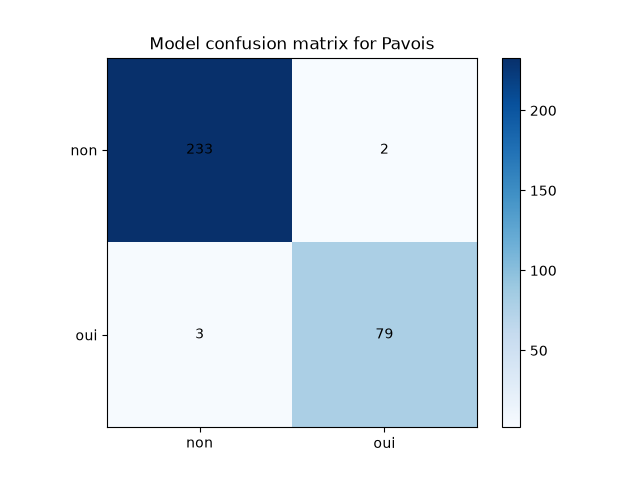
\includegraphics[width=0.65\textwidth]{cmat_s92_b16_e8_c13.png}
    \caption{Matrice de confusion pour la propriété "Pavois", avec des batches de 16 images}
    \label{fig:curve_alpha}
\end{figure}

On remarque ici que le modèle prédit tout le temps le même label, car il n'y a pas assez de donnée dans le label "oui", ce qui donne une bonne précision 52/57 = 91\%, alors qu'en fait il est mauvais.

\end{document}